\section{Household Decisions in a Two-Period Model}
In this section, we solve the household's problem with two periods to gain intuition. 


\paragraph{Period-2 decisions}\label{sec:period2}
Households do not invest in human capital or physical capital in the last period. The only relevant decision is whether to work. 

The household works $n=1$ if and only if $z\geq\overline{z}(h,a)$, with $\overline{z}(h,a) $ defined as 
\begin{equation}
    \ln(w\overline{z}(h,a)x(h)+(1+r)a)-\chi_n = \ln((1+r)a)
\end{equation}
The household faces a trade-off between earning labor income and incurring the disutility of working. 
Given the sector-specific productivity $x(h)$ specified in (\ref{eq:x}), the threshold for idiosyncratic productivity, $\overline{z}(h,a)$, takes on three possible values:
\begin{align}
    \label{eq:z-period2}
\overline{z}(h,a)&=\left \{ 
\begin{array}{cl}
\overline{z}(a)\frac{1}{1-\lambda}  & \text{if }h<h_{M} \\ 
\overline{z}(a) & \text{if }h_{M} \leq h<h_{H} \\ 
\overline{z}(a)\frac{1}{1+\lambda}   & \text{if }h>h_{H}%
\end{array}%
\right. \\
\text{where }\overline{z}(a)&:=\frac{(\exp(\chi_n)-1)(1+r)a}{w}
\end{align}
Households with higher human capital is more likely to work, whereas households with higher physical capital is less likely to work. 

\paragraph{Period-1 decisions}\label{sec:period1}
In addition to labor supply, period-1 decisions include saving and human capital investment, both of which are forward-looking and affected by the idiosyncratic risk associated with the productivity shock $z'$. 
Our model also features a trade-off between human capital investment and labor supply as a working household cannot devote the highest level of effort $e_H$ in human capital investment. Therefore, human capital investment grants households the possibility of a discrete wage hike in the future but may entail a wage loss in the current period. 

To see the implication of this trade-off and how it interacts with uninsured idiosyncratic risk, we proceed in two steps. We first derive the period-1 decisions without uncertainty by assuming that $z'$ is known to the household at period 1 and $z'$ is such that the household will work in period 2. We then reintroduce uncertainty in $z'$ and compare the decision rules with the case without uncertainty.


\subsection{Period-1 Labor Supply and Human Capital Investment} 
\subsubsection{Consumption and saving without uncertainty}

The additive separability of household's utility implies that labor supply $n$ and human capital investment $e$ enters in consumption and saving choices only via the intertemporal budget constraint:
\begin{align*}
    c + \frac{c'}{1+r'}&=(1+r)a+n(wzx(h))+\frac{w'z'x(h')}{1+r'} \\
    \text{with } h'&=ze+ (1-\delta)h.
\end{align*}
The log utility in consumption implies the optimality condition:
\begin{equation}\label{eq:c'}
     c'=\beta(1+r')c.
\end{equation}
Combining it with the budget constraint, we obtain the optimal consumption as a function of labor supply $n$ and human capital investment $e$:
\begin{equation}\label{eq:c}
    c(n,e)=\frac{1}{1+\beta}\left[(1+r)a+n(wzx(h))+\frac{w'z'x\left(h'=ze+ (1-\delta)h\right)}{1+r'} \right].
\end{equation}

\subsubsection{Labor supply and human capital investment}

The optimal consumption rules in (\ref{eq:c}) and (\ref{eq:c'}) allow us to express the household’s problem as the maximization of an objective function in labor supply $n$ and human capital investment $e$:\footnote{This follows since $c' = \beta(1+r')c$, so $\ln c' = \ln\beta + \ln(1+r') + \ln c$.} 
\begin{equation}
   \max_{n,e} (1+\beta)\ln c(n,e) - \chi_n n - \chi_e e
\end{equation}
This maximization depends critically on the household's current human capital and achievable next-period human capital. Accordingly, we partition households into five ranges of $h$: $[0,h_M)$, $[h_M,h_M(1-\delta)^{-1})$, $[h_M(1-\delta)^{-1},h_H)$, $[h_H,h_H(1-\delta)^{-1})$, and $[h_H(1-\delta)^{-1},h_{\max}]$. 

\bigskip
\noindent
We now derive the decision rules for households $h\in[h_M,h_M(1-\delta)^{-1})$ in detail, as the decision rules for the other four ranges are similar.
For households with $h<h_M(1-\delta)^{-1}$, we define two cutoffs in $z$:
\begin{equation}\label{eq:zm}
    \underline{z}_M(h):=\frac{h_M-(1-\delta)h}{e_H}; \overline{z}_M(h):=\frac{h_M-(1-\delta)h}{e_L} 
\end{equation}
These cutoffs divide households into three groups based on their ability to be employed in the middle sector in the next period.

\paragraph{Non-learners} are households with $z < \underline{z}_M(h)$. They cannot achieve $h' > h_M$ with either $e_L$ or $e_H$ level of human capital investment today. As a result, they will choose not to invest in human capital, $e=0$, and their future sectoral productivity will be $x(h')=1-\lambda$. 
These non-learners work $n=1$ if and only if $z\geq \overline{z}^L_{non}(a)$:
\begin{align}
\overline{z}^L_{non}(a)=\frac{(\exp(\frac{\chi_n}{1+\beta})-1)[(1+r)a+\frac{w'z'(1-\lambda)}{1+r'}]}{w}  \label{eq:z-non}
\end{align}

\paragraph{Slow learners} are households with $z \in (\underline{z}_M(h), \overline{z}_M(h))$. These households can reach $h' > h_M$ in the next period only by investing $e = e_H$ today. Their choice is restricted to $e=0$ or $e=e_H$, since selecting $e=e_L$ incurs a cost without any future benefit. Slow learners must trade off between working and human capital investment: choosing $e=e_H$ requires not working today ($n=0$), while opting to work means forgoing investment in human capital ($n=1, e=0$).\footnote{The choice between $(n=0,e=e_H)$ and $(n=0,e=0)$ does not depend on $z$. For $e_H$ to be relevant, $\lambda$ must be large enough so that $(n=0,e=e_H)$ is preferred to $(n=0,e=0)$. See the Appendix for details on the lower bound for $\lambda$.}

Slow learners prefer $(n=1,e=0)$ to $(n=0,e=e_H)$ if and only if $z \geq \overline{z}^L_{slow}(a)$:
\begin{align} 
\overline{z}^L_{slow}(a)=\frac{(\exp(\frac{\chi_n-\chi_e e_H}{1+\beta})-1)[(1+r)a+\frac{w'z'}{1+r'}]+\lambda\frac{w'z'}{1+r'}}{w} \label{eq:z-slow}
\end{align}

\paragraph{Fast learners} are households with $z > \overline{z}_M(h)$. They can achieve $h' > h_M$ in the next period if they invest $e = e_L$ today. In this case, there is no need to exert high effort $e_H$ in human capital investment. The fast learners choose among three options: $(n=1,e=0)$, $(n=1,e=e_L)$, and $(n=0,e=e_L)$.\footnote{Similar to the case of slow learners, the choice between $(n=0,e=e_L)$ and $(n=0,e=0)$ does not depend on $z$. Moreover, since our model is set up so that $(n=0,e=e_H)$ dominates $(n=0,e=0)$, it implies that $(n=0,e=e_L)$ dominates $(n=0,e=0)$. }

The decision rule for fast learners are as follows:
\begin{equation}
n(z,h,a),e(z,h,a) =\left \{ 
\begin{array}{cl}
n=1,e=0  & \text{ if } z \geq \overline{z}^L_{fast}(a) \\
n=1,e=e_L & \text{ if } \underline{z}^L_{fast}(a) \leq z<\overline{z}^L_{fast}(a) \\
n=0,e=e_L & \text{ if } z<\underline{z}^L_{fast}(a)
\end{array}%
\right.
\end{equation}
where 
\begin{align}
\overline{z}^L_{fast}(a)=\frac{\left\{\exp(\frac{\chi_e e_L}{1+\beta})\lambda\left[\exp(\frac{\chi_e e_L}{1+\beta})-1\right]^{-1}-1\right\}\frac{w'z'}{1+r'}-(1+r)a}{w}  \label{eq:z-fast-upper}
\end{align}
\begin{align}
\underline{z}^L_{fast}(a)=\frac{(\exp(\frac{\chi_n}{1+\beta})-1)[(1+r)a+\frac{w'z'}{1+r'}]}{w} \label{eq:z-fast-lower}
\end{align}
We set up our model so that $\overline{z}^L_{fast}(a)>\underline{z}^L_{fast}(a)$.\footnote{Appendix~\ref{app:cutoff_ranking} provides the parameter restrictions such that the condition for $(n=0,e=e_H)$ to dominate $(n=0,e=0)$ is sufficient for $\overline{z}^L_{fast}(a)>\underline{z}^L_{fast}(a)$.} 

\begin{figure}
    \centering
    
\documentclass{standalone}
\usepackage{tikz}
\begin{document}
 % Make the whole figure wider (x-direction).
 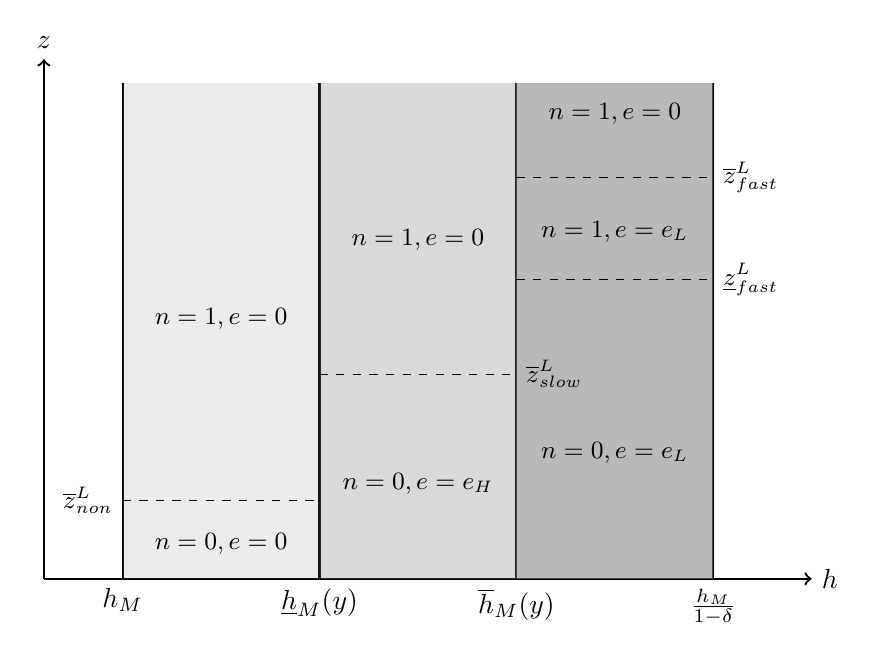
\begin{tikzpicture}[xscale=1.25]

% Decision rule conditional on a given y:
% x-axis: h in [h_M, h_M/(1-delta))
% y-axis: z

% Axes
\draw[thick,->] (-0.8,0) -- (7,0) node[right] {$h$};
\draw[thick,->] (-0.8,0) -- (-0.8,6.6) node[above] {$z$};

% h-range boundaries
\draw[thick] (0,0) -- (0,6.3);
\node[below] at (0,0) {$h_M$};
\draw[thick] (6,0) -- (6,6.3);
\node[below] at (6,0) {$\frac{h_M}{1-\delta}$};


% Learner-type cutoffs in h conditional on y (schematic placement)
\draw[thick] (2,0) -- (2,6.3);
\draw[thick] (4,0) -- (4,6.3);
\node[below] at (2,0) {$\underline{h}_M(y)$};
\node[below] at (4,0) {$\overline{h}_M(y)$};

% Shade learner-type regions (conditional on y)
\fill[gray, opacity=0.15] (0,0) rectangle (2,6.3); % non-learners
\fill[gray, opacity=0.30] (2,0) rectangle (4,6.3); % slow learners
\fill[gray, opacity=0.55] (4,0) rectangle (6,6.3); % fast learners

% z cutoffs (schematic heights)
\def\zNon{1.0}
\def\zSlow{2.6}
\def\zFastL{3.8}
\def\zFastU{5.1}

% Non-learner cutoff
\draw[dashed] (0,\zNon) -- (2,\zNon);
\node[left] at (0,\zNon) {\small $\overline{z}^L_{non}$};

% Slow-learner cutoff
\draw[dashed] (2,\zSlow) -- (4,\zSlow);
\node[right] at (4,\zSlow) {\small $\overline{z}^L_{slow}$};

% Fast-learner cutoffs
\draw[dashed] (4,\zFastL) -- (6,\zFastL);
\draw[dashed] (4,\zFastU) -- (6,\zFastU);
\node[right] at (6,\zFastL) {\small $\underline{z}^L_{fast}$};
\node[right] at (6,\zFastU) {\small $\overline{z}^L_{fast}$};

% Decision labels inside regions
% Non-learners
\node at (1,0.45) {\small $n=0,e=0$};
\node at (1,3.3) {\small $n=1,e=0$};

% Slow learners
\node at (3,1.2) {\small $n=0,e=e_H$};
\node at (3,4.3) {\small $n=1,e=0$};

% Fast learners
\node at (5,1.6) {\small $n=0,e=e_L$};
\node at (5,4.4) {\small $n=1,e=e_L$};
\node at (5,5.9) {\small $n=1,e=0$};

\end{tikzpicture}

\end{document}

\caption{Decision Rule Diagram for $h_M \leq h<h_M(1-\delta)^{-1}$}
\begin{flushleft}
\footnotesize{The human capital $h$ changes along the horizontal line and the idiosyncratic productivity $z$ changes along the vertical line. The two diagonal lines, $\overline{z}_M(h)$ and $\underline{z}_M(h)$, separate the state space into three areas: the unshaded area represents the non-learners, the lightly-shaded area represents the slow learners, and the darkly-shaded  area represents the fast learners. The areas are divided by four dashed horizontal lines associated with cutoffs $\overline{z}^L_{non}$, $\overline{z}^L_{slow}$, $\underline{z}^L_{fast}$, and $\overline{z}^L_{fast}$ that are functions of capital holding $a$.} 
\end{flushleft}
    
\label{fig:rule-diagram}
\end{figure}

\paragraph{Decision rule diagram:}Figure \ref{fig:rule-diagram} illustrates the decision rule $(n,e)$ as a function of states $(z,h,a)$ for households with $h_M \leq h<h_M\frac{1}{1-\delta}$. The human capital $h$ changes along the horizontal line and the idiosyncratic productivity $z$ changes along the vertical line. The two diagonal lines, $\overline{z}_M(h)$ and $\underline{z}_M(h)$ defined in (\ref{eq:zm}), separate the state space into three areas: the unshaded area represents the non-learners, the lightly-shaded area represents the slow learners, and the darkly-shaded area represents the fast learners. The areas are divided by four dashed horizontal lines associated with cutoffs $\overline{z}^L_{non}(a)$, $\overline{z}^L_{slow}(a)$, $\underline{z}^L_{fast}(a)$, and $\overline{z}^L_{fast}(a)$ that are functions of capital holding $a$ and defined in (\ref{eq:z-non}), (\ref{eq:z-slow}), (\ref{eq:z-fast-lower}), and (\ref{eq:z-fast-upper}).


This decision rule diagram is representative for households in other four ranges of human capital. Figure \ref{fig:e-digram} illustrates the regions in which households make positive human capital investments. Striped shading highlights where investment occurs, with dark areas denoting fast learners and light areas representing slow learners. 

For households with $h<h_M$, $\overline{z}_M(h)$ and $\underline{z}_M(h)$ continue to be the boundaries that separate non-learners, slow learners and fast learners, but the four cutoffs are $\overline{z}^L_{non}\frac{1}{1-\lambda}$, $\overline{z}^L_{slow}\frac{1}{1-\lambda}$, $\underline{z}^L_{fast}\frac{1}{1-\lambda}$, and $\overline{z}^L_{fast}\frac{1}{1-\lambda}$.

For households with $h_M\frac{1}{1-\delta} \leq h<h_H\frac{1}{1-\delta}$, the boundaries for state space division change to $\overline{z}_H(h)$ and $\underline{z}_H(h)$:
\begin{equation}\label{eq:zh}
    \underline{z}_H(h):=\frac{h_H-(1-\delta)h}{e_H}; \qquad \overline{z}_H(h):=\frac{h_H-(1-\delta)h}{e_L} 
\end{equation}
If $h_M\frac{1}{1-\delta} \leq h<h_H$, the four cutoffs that partition the decision regions for households are denoted as $\overline{z}^M_{non}(a)$, $\overline{z}^M_{slow}(a)$, $\underline{z}^M_{fast}(a)$, and $\overline{z}^M_{fast}(a)$ (see Appendix~\ref{app:cutoff_formulae} for the explicit formulae).\footnote{Appendix~\ref{app:cutoff_ranking} provides parameter restrictions for $\overline{z}^M_{fast}(a)>\underline{z}^M_{fast}(a)$.}
If $h_H \leq h<h_H\frac{1}{1-\delta}$, the analogous cutoffs are given by $\overline{z}^M_{non}\frac{1}{1+\lambda}$, $\overline{z}^M_{slow}\frac{1}{1+\lambda}$, $\underline{z}^M_{fast}\frac{1}{1+\lambda}$, and $\overline{z}^M_{fast}\frac{1}{1+\lambda}$.


Households with $h \geq h_H\frac{1}{1-\delta}$ are always non-learners, since their human capital guarantees high-sector employment next period without further investment. For them, only the cutoff $\overline{z}^H_{non}(a)\frac{1}{1+\lambda}$ matters.

\begin{figure}
    \centering
    
\documentclass{standalone}
\usepackage{tikz}
\usetikzlibrary{patterns}
\begin{document}
\begin{tikzpicture}

% Axes
\draw[thick,->] (-1,0) -- (11,0) node[right] {$h$};
\draw[thick,->] (-1,0) -- (-1,6.6) node[above] {$z$};

% Key h cutoffs
\draw[thick] (2,0) -- (2,6.3);
\node[below] at (2,0) {$h_M$};
\draw[thick] (4.5,0) -- (4.5,6.3);
\node[below] at (4.5,0) {$\frac{h_M}{1-\delta}$};
\draw[thick] (7.5,0) -- (7.5,6.3);
\node[below] at (7.5,0) {$h_H$};
\draw[thick] (10,0) -- (10,6.3);
\node[below] at (10,0) {$\frac{h_H}{1-\delta}$};

% h-cutoffs conditional on y (schematic placement, labels carry the economics)
% Relative to h_M
\draw[thick] (1.2,0) -- (1.2,6.3);
\draw[thick] (3.2,0) -- (3.2,6.3);
\node[below] at (1.2,0) {\scriptsize $\underline{h}_M(y)$};
\node[below] at (3.2,0) {\scriptsize $\overline{h}_M(y)$};
% Relative to h_H
\draw[thick] (6.0,0) -- (6.0,6.3);
\draw[thick] (8.8,0) -- (8.8,6.3);
\node[below] at (6.0,0) {\scriptsize $\underline{h}_H(y)$};
\node[below] at (8.8,0) {\scriptsize $\overline{h}_H(y)$};

% Grey shading: learner types (conditional on y), by h
% Left block (threshold h_M): [0,4.5]
\fill[gray, opacity=0.15] (0,0) rectangle (1.2,6.3);  % non-learners
\fill[gray, opacity=0.30] (1.2,0) rectangle (3.2,6.3); % slow learners
\fill[gray, opacity=0.55] (3.2,0) rectangle (4.5,6.3); % fast learners
% Right block (threshold h_H): [4.5,10]
\fill[gray, opacity=0.15] (4.5,0) rectangle (6.0,6.3);  % non-learners
\fill[gray, opacity=0.30] (6.0,0) rectangle (8.8,6.3);  % slow learners
\fill[gray, opacity=0.55] (8.8,0) rectangle (10,6.3);   % fast learners

% Stripes: region where e>0 (schematic, uses z cutoffs)
% Define schematic z cutoffs
\def\zSlowL{2.6}   % \overline{z}^L_{slow}
\def\zFastL{5.1}   % \overline{z}^L_{fast}
\def\zSlowM{2.2}   % \overline{z}^M_{slow}
\def\zFastM{4.6}   % \overline{z}^M_{fast}

% Left block: investment for slow learners (e_H) when z is low
\fill[pattern=north east lines, pattern color=black, opacity=0.35]
  (1.2,0) rectangle (3.2,\zSlowL);
% Left block: investment for fast learners (e_L) when z is below \overline{z}^L_{fast}
\fill[pattern=north east lines, pattern color=black, opacity=0.35]
  (3.2,0) rectangle (4.5,\zFastL);

% Right block: investment for slow learners (e_H) when z is low
\fill[pattern=north east lines, pattern color=black, opacity=0.35]
  (6.0,0) rectangle (8.8,\zSlowM);
% Right block: investment for fast learners (e_L) when z is low
\fill[pattern=north east lines, pattern color=black, opacity=0.35]
  (8.8,0) rectangle (10,\zFastM);

% Dashed horizontal cutoff lines (labels)
\draw[dashed] (1.2,\zSlowL) -- (3.2,\zSlowL);
\node[left] at (-1,\zSlowL) {\scriptsize $\overline{z}^L_{slow}$};
\draw[dashed] (3.2,\zFastL) -- (4.5,\zFastL);
\node[left] at (-1,\zFastL) {\scriptsize $\overline{z}^L_{fast}$};
\draw[dashed] (6.0,\zSlowM) -- (8.8,\zSlowM);
\node[left] at (-1,\zSlowM) {\scriptsize $\overline{z}^M_{slow}$};
\draw[dashed] (8.8,\zFastM) -- (10,\zFastM);
\node[left] at (-1,\zFastM) {\scriptsize $\overline{z}^M_{fast}$};

% Legend (minimal)
\node[anchor=west] at (-0.8,6.35) {\scriptsize grey: learner type (conditional on $y$)};
\node[anchor=west] at (4.9,6.35) {\scriptsize stripes: $e>0$ region};

\end{tikzpicture}
\end{document}


\caption{State Space for Human Capital Investment}
\begin{flushleft}
\footnotesize{The darkly-shaded striped areas indicate the state space for human capital investment equal to $e_L$ by the fast learners. The lightly-shaded striped areas indicate the state space for human capital investment equal to $e_H$ by the slow learners.} 
\end{flushleft}
    
\label{fig:e-digram}
\end{figure}





\subsection{The Effects of Uninsured Idiosyncratic Risk}
We now reintroduce the idiosyncratic risk to households in period 1 by assuming that $z'$ follows a log-normal distribution with mean $\overline{z}'$ and variance $\sigma^2_z$. 

Our previous analysis without uncertainty is a special case with $\sigma^2_z=0$. The effects of uninsured idiosyncratic risk can be thought as how households' decisions change when the distribution of $z'$ undergoes a mean-preserving spread in the sense of second-order stochastic dominance.

From a consumption-saving perspective, the uncertain $z'$ is associated with future labor income risk. It is well understood in the literature that idiosyncratic future income risk raises the expected marginal utility of future consumption for households with log utility and makes them save more. In our model, households can also supply more labor to mitigate the effect of idiosyncratic income risk on the marginal utility of consumption. 

From the perspective of human capital investment, the uncertain $z'$ is associated with risk in the return to human capital. Conditional on working, households' income increases with $z'$: $c'=(1+r')a'+w'x(h')z'$. $\ln(c')$ is increasing and concave in $z'$, and a higher $x(h')$ increases the concavity.\footnote{The marginal effect of $z'$ on $\ln(c')$ is 
\begin{equation*}
    \frac{\partial\ln(c')}{\partial z'}=\frac{w'x(h')}{(1+r')a'+w'x(h')z'} > 0
\end{equation*}
The second derivative is 
\begin{equation*}
    \frac{\partial^2\ln(c')}{(\partial z')^2}=-\left[\frac{w'x(h')}{(1+r')a'+w'x(h')z'}\right]^2 <0
\end{equation*}
and is more negative if $x(h')$ is higher.} Consider two levels of $h'$, $\overline{h'}>\underline{h'}$, a mean-preserving spread of $z'$ distribution reduces the expected utility at both levels of $h'$ but the reduction is larger for the higher level $\overline{h'}$. Hence, the expected utility gain of moving from $\underline{h'}$ to $\overline{h'}$ is smaller due to the idiosyncratic risk. Human capital investment is discouraged.

Taking into account endogenous labor supply reinforces the discouragement of human capital investment by the idiosyncratic risk. Recall from Section \ref{sec:period2} that households with $z'$ lower than a cutoff do not work. The endogenous labor supply therefore provides insurance against the lower tail risk of the idiosyncratic $z'$. Moreover, the cutoff in $z'$ is lower for those with higher human capital $h'$. This makes households with higher $h'$ more exposed to the lower tail risk than those with lower $h'$, further reducing the gain of human capital investment.


\begin{proposition}
    The uninsured idiosyncratic risk in $z'$ makes households in period 1 save more, work more and invest less in human capital.
\end{proposition}


\subsection{Period-1 Saving and Human Capital Investment}\label{sec:saving}
In this section, we study the impact of endogenous human capital investment on households’ saving decisions. Specifically, we compare optimal saving behavior in two scenarios: one in which households can choose to invest in human capital, and an alternative scenario in which human capital is exogenously fixed. To facilitate the comparison, we assume in this section that there is no human capital depreciation.\footnote{If depreciation is allowed, the analysis proceeds similarly but involves more comparison paris.}

When the optimal choice of human capital investment is zero, optimal saving is identical in both scenarios. When the optimal human capital investment is either $e_L$ or $e_H$, we compare the household's optimal saving to the case where human capital investment is exogenously fixed at zero, i.e., $(n=1, e=0)$.\footnote{Why not compare to $(n=0,e=0)$? Such a comparison is not meaningful when considering $(n=1, e=e_L)$ because the two scenarios involve different state spaces. To see it, suppose conditions are 
such that $(n=1,e=e_L)$ is optimal. If we were to fix $e=0$ 
exogenously, the household’s lifetime income would fall, 
and as a result the household would have a greater 
incentive to work. Thus, it is not possible for the 
household to deviate from choosing $n=1$ when human capital 
is held fixed at $e=0$. The comparison between $(n=0,e=0)$ 
and $(n=0,e=e_L \text{ or } e_H)$ is similar to the 
comparison between $(n=1,e=0)$ to $(n=1,e=e_L)$, since human capital investment does not affect period-1 labor income in either case.}

To make the human captial relevant, we assume that $n'=1$ in period 2. The additive separability of work and human capital investment effort from consumption allows us to consider the optimal saving conditional on a given choice of labor supply and human capital investment. 

In particular, the household maximizes expected lifetime utility:   
\begin{equation}\label{eq:savingprob}
\max_{a'} : \ln(c) + \beta \mathbb{E}_{z'}[\ln(c')],
\end{equation}
subject to the budget constraints
\begin{align}
c + a' &= (1+r)a + n(wzx(h)) , \\
c' &= (1+r')a' + w'z'x(h'), \\
\text{with } h' &= ze + (1-\delta)h, e \in \{0, e_L, (1-n)e_H\}
\end{align}

\subsubsection{Effect of on-job-training on saving}\label{sec:on-job-saving}
We now compare the optimal saving between $(n=1,e=e_L)$ and $(n=1,e=0)$, where $e_L$ allows households to move to a higher sector in period 2 with higher sectoral productivity $x(h')$. 

To simplify the notation while maintaining the key economic forces, we normalize $(1+r)=(1+r')= 1$, $w=w'= 1$, the period-1 productivity shock $z=1$ and the period-2 productivity shock $z'$ to $\ln z' \sim \mathcal{N}(0,\sigma_z^2)$. The budget constraints become:
\begin{equation}
c + a' = a + x , \quad c' = a' + txz'
\end{equation}
where $x$ is the household's period-1 labor income that reflects both productivity and skill. $t\geq 1$ represents the effect of human capital investment on period-2 income: $t>1$ if $e=e_L$; $t=1$ if $e=0$.

The optimal saving is determined by the FOC:
\begin{equation}
\frac{1}{a+x-a'} = \beta\mathbb{E}_{z'}\big(\frac{1}{a'+txz'}\big)
\end{equation}
Denoting the mean and variance of $z'$ as $\mu$ and $\Sigma$, respectively:
\begin{equation}
    \mu \equiv \mathbb{E}[z'] = e^{\sigma_z^2/2}, \quad \Sigma \equiv\operatorname{Var}(z') = e^{\sigma_z^2}(e^{\sigma_z^2}-1).
\end{equation}
The second-order approximate solution to the FOC is:
\begin{equation}
a'^*(x,a;t) = \underbrace{\frac{\beta(a+x) - tx\mu}{1+\beta}}_{\text{CE}} + \underbrace{\frac{t^2x^2\Sigma}{\beta(a+x + tx\mu)}}_{\text{Precautionary}}
\end{equation}
The first term is the \textit{certainty-equivalent} saving, which reflects the consumption smoothing motive, increasing in the period-1 resources $a+x$ and decreasing in the period-2 expected labor income $tx\mu$. The second term is the \textit{precautionary} saving, which is increasing in the variance of period-2 labor income $t^2x^2\Sigma$ and decreasing in the expected total resources $a+x+tx\mu$.

The effect of on-job-training on saving can be decomposed into two components:
\begin{equation}
    \frac{\partial a'^\star}{\partial t}(x,a;t)
    = -\frac{x\mu}{1+\beta}+\frac{x^2 \Sigma}{\beta}\frac{t\,[2(a+x) + t x \mu]}{(a+x + t x \mu)^2}.
    \label{eq:dadt_partial}
\end{equation}
The first term being negative captures the \textit{crowd-out} effect on saving via consumption-smoothing motive as on-job-training increases the expected period-2 labor income $tx\mu$. The second positive term captures the \textit{crowd-in} effect via precautionary saving motive as on-job-training exposes households to larger future income risk.

To capture the overall impact of on-job-training on saving, we define:
\begin{equation} \label{eq:dadt_integral}
    \Delta_{\text{on-job}}(x,a;t) = a'^\star(x,a;t) - a'^\star(x,a;1) = \int_1^t \frac{\partial a'^\star}{\partial u}(x,a;u) du,
\end{equation}
where $a'^\star(x,a;t)$ is the optimal saving when households undertake on-job-training, and $a'^\star(x,a;1)$ is the optimal saving when human capital is kept exogenously fixed. 

Whether on-job-training increases or decreases saving ultimately depends on the balance between the crowd-out effect (via higher expected future income) and the precautionary crowd-in effect (via heightened future income risk). The next proposition demonstrates that these effects can dominate differently depending on period-1 income $x$, so that the overall impact of on-job-training on saving can differ between low- and high-income households.



\begin{proposition}\label{prop:dadt}
    If the idiosyncratic risk is large enough, i.e., $\frac{\Sigma}{\mu}>\sigma^*(t)$, on-job-training crowds out saving for low-income households and crowds in saving for high-income households: 
    for $x<x^\ast(a,t)$, $e=e_L$ lowers saving $\Delta_{\text{on-job}}(x,a;t)<0$; for $x>x^\ast(a,t)$, $e=e_L$ raises saving $\Delta_{\text{on-job}}(x,a;t)>0$.
\end{proposition}
\begin{proof}
    See Appendix~\ref{appsec: proofs}.
\end{proof}


\subsubsection{Effect of full-time training on saving}
We next compare the optimal saving between $(n=0,e=e_L \text{ or } e_H)$ and $(n=1,e=0)$. Note that  full-time training requires the households to give up their labor income in period 1, which is not the case for on-job-training. Following the same normalization and notation as in the previous subsection, we can write the budget constraints with full-time training and without training as:
\begin{align}
e=e_H: \quad c + a' &= a, \quad c' = a' + txz'\\
e=0: \quad c + a' &= a + x, \quad c' = a' + xz'
\end{align}
where $t>1$ captures the effect of full-time training on period-2 income. 

The second-order approximation to the optimal saving problem yields:
\begin{align}
    e = e_H: \quad a'^*_{e_H}(x,a;t) &= \underbrace{\frac{\beta a - t x \mu}{1+\beta}}_{\text{CE}} + \underbrace{\frac{t^2 x^2 \Sigma}{\beta(a + t x \mu)}}_{\text{Precautionary}} \\
    e = 0: \quad a'^*(x,a;1) &= \underbrace{\frac{\beta(a + x) - x \mu}{1+\beta}}_{\text{CE}} + \underbrace{\frac{x^2 \Sigma}{\beta(a + x + x \mu)}}_{\text{Precautionary}}
\end{align} 
The overall effect of full-time training on saving can be expressed as:
\begin{align}
    \Delta_{\text{full-time}}(x,a;t) &= a'^*_{e_H}(x,a;t) - a'^*(x,a;1) \notag \\
    &= \Delta_{\text{on-job}}(x,a;t) + \Delta_H(x,a;t) \\
    \text{where } \Delta_H(x,a;t) &\equiv x \Bigg[ -\frac{\beta}{1+\beta} + \frac{\Sigma}{\beta} \frac{t^2 x^2}{(a + x + t x \mu)(a + t x \mu)} \Bigg] \label{eq:dadt_fulltime}
\end{align}
Here, $\Delta_H(x,a;t)$ captures the additional impact of full-time training on saving, over and above that of on-job-training. The first term reflects a further reduction in saving due to the need to forgo period-1 labor income. The second term shows an increase in precautionary saving, as reduced current resources limit households’ ability to self-insure against idiosyncratic risk in period 2.

The following lemma establishes some properties of $\Delta_H(x,a;t)$:
\begin{lemma}\label{lem:fulltime}
    If $\frac{\Sigma}{\mu}<\hat{\sigma}(t)$, $\Delta_H(x,a;t)<0$ and decreases in $x$. If $\frac{\Sigma}{\mu}>\overline{\sigma}(t)$, $\Delta_H(x,a;t)>0$ if and only if $x>\hat{x}(a,t)$; moreover, for $x>\hat{x}(a,t)$, $\Delta_H(x,a;t)$ increases in $x$.
\end{lemma}
\begin{proof}
    See Appendix~\ref{appsec: proofs}.
\end{proof}

\noindent Taken together, Proposition \ref{prop:dadt} and Lemma \ref{lem:fulltime} imply that, when the idiosyncratic risk is large enough, full-time training \textit{crowds out} saving for low-income households, but \textit{crowds in} saving for high-income households.
\begin{proposition}\label{prop:fulltime}
If the idiosyncratic risk is large enough, i.e., $\frac{\Sigma}{\mu}>\max\{\sigma^*(t),\hat{\sigma}(t)\}$, full-time training crowds out saving for low-income households and crowds in saving for high-income households: 
    for $x<\min\{x^*(a,t),\hat{x}(a,t)\}$, $e=e_H$ lowers saving $\Delta_{\text{full-time}}(x,a;t)<0$; for $x>\max\{x^*(a,t),\hat{x}(a,t)\}$, $e=e_H$ raises saving $\Delta_{\text{full-time}}(x,a;t)>0$.
\end{proposition}

\subsection{The Effects of an Anticipated Period-2 AI Shock}
Suppose that an AI shock is anticipated to occur in period 2 and to increase the labor productivity for the low sector and the high sector but not the middle sector. The effect of AI shock on the sectoral productivity is captured by $\gamma$ with $0<\gamma<1$:
\begin{equation}
    \label{eq:xAI}
x(h')=\left \{ 
\begin{array}{cl}
1-\lambda + \gamma \lambda & \text{low sector if }h'<h_{M} \\ 
1 & \text{middle sector if }h_{M}<h'<h_{H} \\ 
1+\lambda + \gamma \lambda & \text{high sector if }h'>h_{H}%
\end{array}%
\right. 
\end{equation}
In other words, the AI shock increases average labor productivity, reduces the earnings premium for the middle sector, and enlarges the earnings premium for the high sector relative to the middle sector.

%\subsubsection{AI's effect on human capital investment and labor supply}

\subsubsection{Effects on human capital investment} 

The AI shock lowers the incentive to work in the middle sector in period 2. Consequently, households with $h < h_M/(1-\delta)$ reduce their human capital investment, while those with $h > h_M/(1-\delta)$ increase it. More specifically, the upper bounds that determine whether households undertake positive human capital investment -- denoted by $\overline{z}^L_{slow}$ and $\overline{z}^L_{fast}$ for $h < h_M/(1-\delta)$, and $\overline{z}^M_{slow}$ and $\overline{z}^M_{fast}$ for $h > h_M/(1-\delta)$ -- respond in opposite directions to the anticipated shock: the former decrease with $\gamma$ and the latter increase. This relationship is formalized below.

\begin{proposition}\label{prop:AI_human_capital}
An anticipated AI shock decreases human capital investment among households with $h < h_M/(1-\delta)$, but increases it among those with $h > h_M/(1-\delta)$. Specifically, $\overline{z}^L_{slow}$ and $\overline{z}^L_{fast}$ decrease with $\gamma$, while $\overline{z}^M_{slow}$ and $\overline{z}^M_{fast}$ increase with $\gamma$.
\end{proposition}
\begin{proof}
    See Appendix~\ref{appsec: proofs}.
\end{proof}

\subsubsection{Effects on labor supply} 
\paragraph{via income:} 
The AI shock raises period-2 labor income for households who will work in the low or high sector, leading to a positive income effect that reduces their labor supply in period 1. 

\paragraph{via full-time training:} Because full-time training and labor supply compete for time, the AI shock affects their tradeoff through its impact on human capital investment incentives. For $h>h_M/(1-\delta)$, where AI makes investing in additional skills more attractive, households are more likely to engage in full-time training and thus reduce period-1 labor supply. In contrast, for $h<h_M/(1-\delta)$, where the AI shock lowers the payoff to investing in skills, households shift away from full-time training and supply more labor in the first period. 


\subsubsection{Effects on saving}

The AI shock increases sectoral labor productivity for the low and high sectors in period 2, while leaving the middle sector's labor productivity unchanged. Its effect on saving can be analyzed as if we are varying the parameter $t$ in the functions $\Delta_{\text{on-job}}(x,a;t)$, defined in \eqref{eq:dadt_integral}, and $\Delta_{H}(x,a;t)$, defined in \eqref{eq:dadt_fulltime}. 

\begin{proposition}\label{prop:Delta}
    $\Delta_{H}(x,a;t)$ is increasing in $t$. $\Delta_{\text{on-job}}(x,a;t)$ is convex in $t$:
    \begin{itemize}
        \item If $\Delta_{\text{on-job}}(x,a;t)>0$ and $t>1$, $\Delta_{\text{on-job}}(x,a;t') > \Delta_{\text{on-job}}(x,a;t)$ for $t'>t>1$. 
        \item If $\Delta_{\text{on-job}}(x,a;t) > 0$ and $t<1$, $\Delta_{\text{on-job}}(x,a;t') < \Delta_{\text{on-job}}(x,a;t)$ for $1>t'>t$.
    \end{itemize}
\end{proposition}
\begin{proof}
    See Appendix~\ref{appsec: proofs}.
\end{proof}


\paragraph{Households who stay in the same sector}
For middle-sector households, the AI shock leaves both their incomes and saving unchanged.

By contrast, low-sector and high-sector households experience an increase in period-2 labor income $x'$ as a result of the AI shock. If they remain in the same sector without needing additional human capital investment or on-the-job training, their saving behavior in the absence of the AI shock can be compared to the scenario with fixed human capital. Following the AI shock, however, their situation resembles one with on-the-job training that enhances $x'$ (i.e., $t>1$). Thus, the effect of the AI shock on saving is captured by the on-the-job training impact, $\Delta_{\text{on-job}}(x,a;t)$.

As shown in Proposition \ref{prop:dadt}, $\Delta_{\text{on-job}}(x,a;t)$ has opposite signs for low-skill and high-skill households. This implies that the AI shock \textit{crowds out} saving among low-sector households, while it \textit{crowds in} saving for high-sector households.

For households who must undertake full-time training to remain in the high sector, $\Delta_{H}(x,a;t)$ captures the additional effect of such training on saving. In this case, a higher $x'$—brought about by the AI shock—corresponds to an increase in $t$, further boosting $\Delta_{H}(x,a;t)$ (Proposition \ref{prop:Delta}). Consequently, the AI shock \textit{crowds in} saving for high-sector households in this scenario as well.


\paragraph{Households who upskill} For low-sector households, saving behavior remains unchanged, as the AI shock does not affect their future productivity after upskilling.

For the middle-sector households who upskill via on-job-training, the AI shock boosts their future productivity gain from $\lambda$ to $(1+\gamma)\lambda$, which corresponds to a higher $t$ in $\Delta_{\text{on-job}}(x,a;t)$ with $t>1$. According to Proposition \ref{prop:Delta}, if the pre-shock effect of on-the-job training on saving is positive, the AI shock will \textit{raise} saving. However, if this effect is negative, the overall impact of the AI shock on saving becomes ambiguous.

For the middle-sector households who upskill via full-time training, there is an \textit{additional positive effect} of the AI shock on their saving, because a higher $x'$ increases $\Delta_{H}(x,a;t)$ (Proposition \ref{prop:Delta}).



\paragraph{Households who downskill} Downskilling, which reflects human capital depreciation, does not require any new investment in skills. For high-sector households who transition downward, the AI shock leaves their future productivity -- and thus their saving -- unchanged.

For middle-sector households who downskill to the low sector, their saving differs from the fixed human capital scenario by $\Delta_{\text{on-job}}(x,a;t)$ with $t<1$. The AI shock mitigates their future productivity loss by reducing it from $\lambda$ to $(1-\gamma)\lambda$, effectively increasing $t$ to a new value $t'<1$. According to Proposition \ref{prop:Delta}, if the pre-shock effect $\Delta_{\text{on-job}}(x,a;t)$ is positive, the AI shock will \textit{reduce} saving. If this effect is negative, however, the overall impact of the AI shock on saving is ambiguous.





\subsection{Limitations of the two-period model}
Up to this point, our analysis has focused on how AI influences household-level decisions regarding human capital investment, labor supply, and saving within the framework of a two-period model. While this provides valuable insights into individual behavioral responses, understanding the broader, economy-wide implications of AI requires moving to a more comprehensive setting -- a quantitative model with an infinite time horizon, endogenous asset accumulation, and general equilibrium feedback.

\paragraph{General equilibrium (GE) effects} When households adjust their investment in human capital, labor supply, and savings in response to AI, these changes aggregate up to affect the total supply of effective labor and capital in the economy. As these aggregates shift, they exert downward or upward pressure on the wage rate and the interest rate, feeding back into each household’s optimization problem. Thus, general equilibrium effects capture the intricate loop by which individual decisions shape, and are shaped by, the macroeconomic environment.

\paragraph{Composition effects} Endogenizing human capital investment injects dynamism into how households sort themselves among the three skill sectors. When an AI shock occurs, individuals may choose to retrain, upskill, or even move to lower-skilled work, reshaping the distribution of labor across sectors. This shifting composition changes the relative size of each sector, with significant consequences for both aggregate outcomes and the distributional effects of AI.
